\documentclass[12pt,a4paper]{scrreprt}
 \usepackage{ngerman}
 \usepackage[utf8]{inputenc}

\usepackage{listings}


 \usepackage[T1]{fontenc}
\usepackage{pdfpages}
\usepackage{url}
\graphicspath{{/Users/Timo/Documents/DHBW/Semester4/Projektarbeit/}}
\usepackage{graphicx}
\usepackage{wrapfig}
\usepackage{geometry} 
\geometry{a4paper, top=25mm, left=25mm, right=25mm, bottom=25mm, headsep=15mm, 
  footskip=12mm}
\usepackage{textcomp}
% Header
\usepackage{fancyhdr}
\pagestyle{fancy}
% Header für Seiten ohne Chapter
\fancyhf{}
\fancyhead[L]{Studienarbeit Timo Höting \\ DHBW Karlsruhe}
   \fancyhead[R]{
\includegraphics[scale=0.3]{./data/dhbwlogo.jpg} } 
\fancyfoot[C]{\thepage}
\fancypagestyle{plain}{
% Header für Seiten mit Chapter
\fancyhf{}
   \fancyhead[L]{Studienarbeit Timo Höting \\ DHBW Karlsruhe}
   \fancyhead[R]{
\includegraphics[scale=0.3]{./data/dhbwlogo.jpg} } 
\fancyfoot[C]{\thepage}
}

\begin{document}
\begin{titlepage}
\begin{figure}
\makebox[\textwidth]{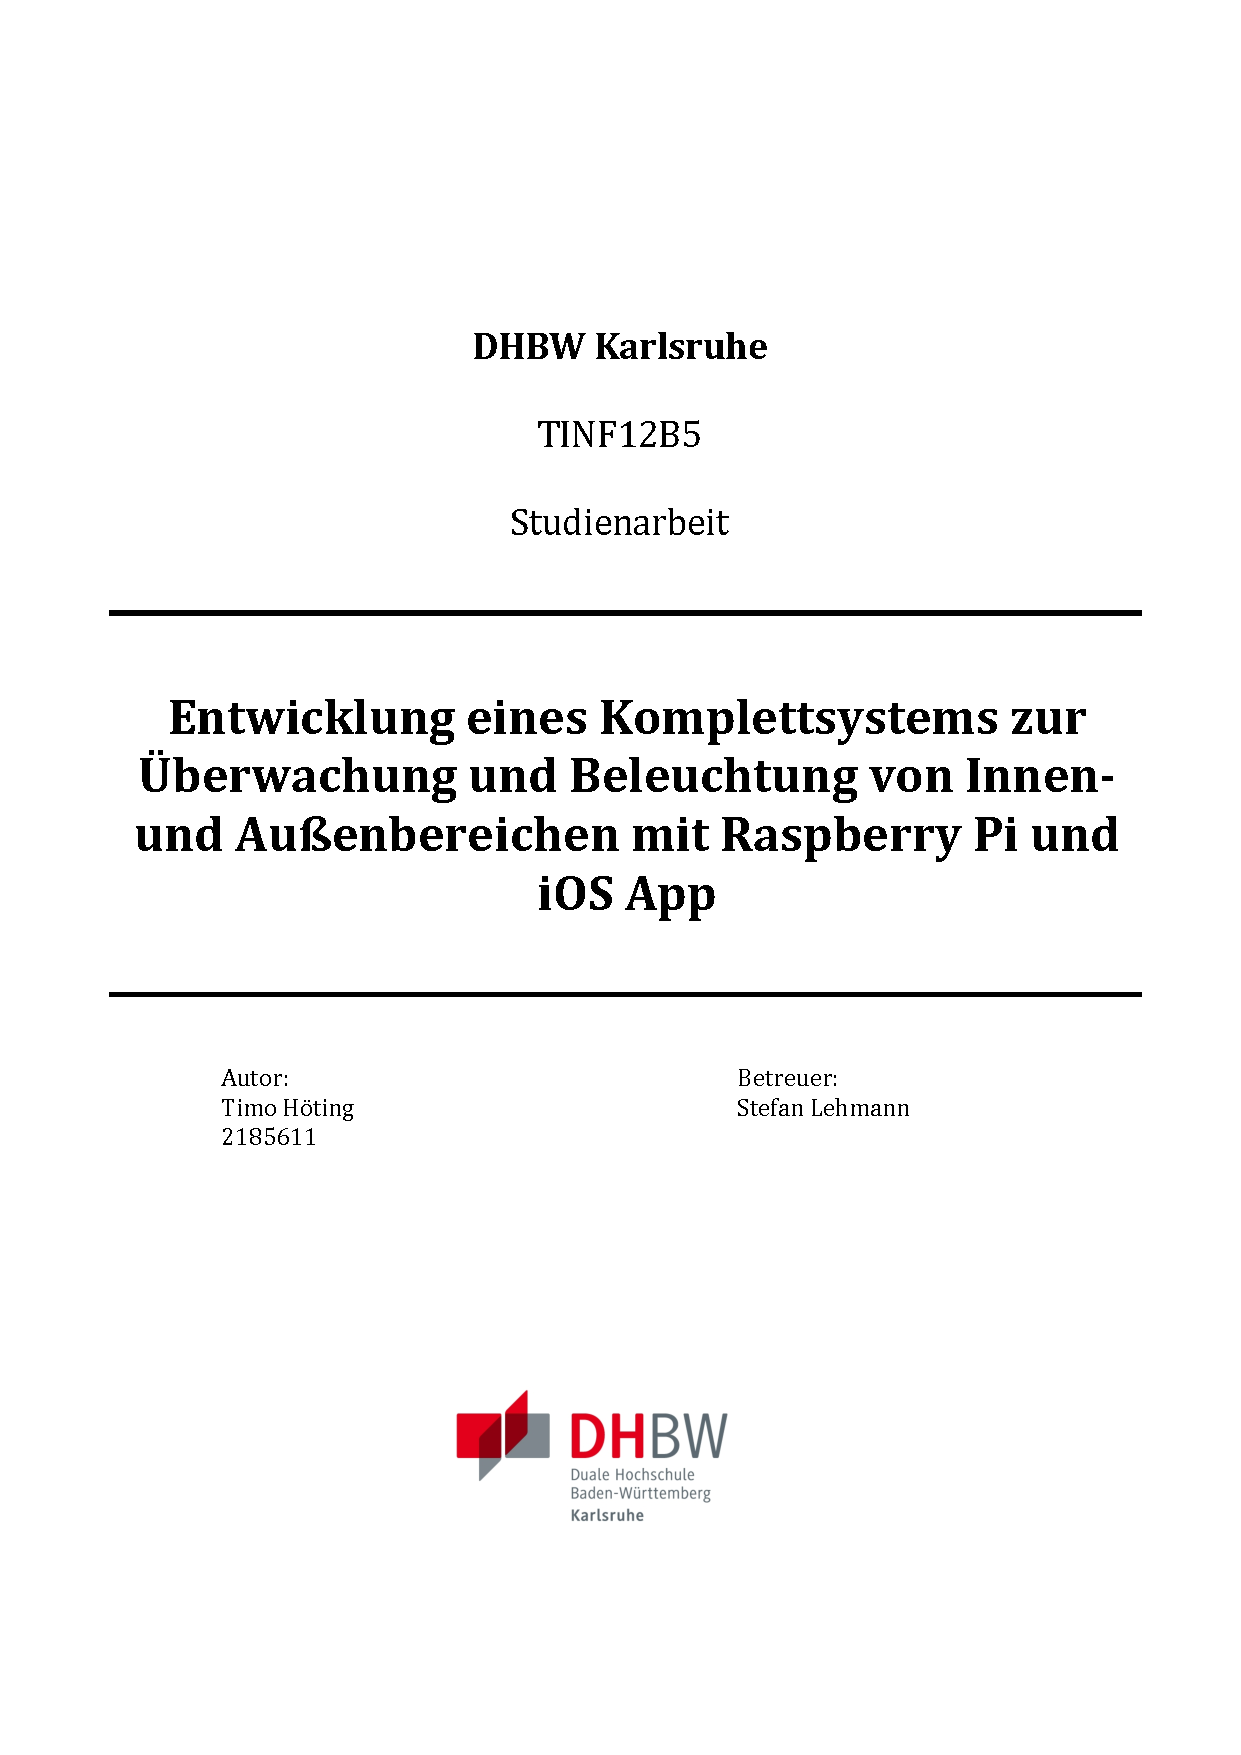
\includegraphics[page={1},width=\paperwidth]{./data/deckblatt.pdf}} \\
\end{figure}
\end{titlepage}
\clearpage
\begin{figure}
\makebox[\textwidth]{\includegraphics[page={2},width=\paperwidth]{./data/deckblatt.pdf}} \\
\end{figure}
\thispagestyle{empty} %Head löschen
\tableofcontents
\thispagestyle{empty}  
\chapter{Einleitung} 
\section{Einleitung}
Diese Studienarbeit wird im Zuge des Studiums Bachelor of Engineering - Informationstechnik an der DHBW Karlsruhe erstellt. \\\\
Im dieser Studienarbeit soll ein Komplettsystem entwickelt werden, dass sowohl die Über- wachung als auch die Steuerung der Beleuchtung von Innen- und Außenbereichen ermög- licht. Das System soll nach der Entwicklung universell einsetzbar und leicht konfigurierbar sein.\\\\
Die Beleuchtung soll mit adressierbaren LED-Pixeln umgesetzt werden, da diese sehr leicht steuer- und erweiterbar sind. Für die Erkennung von Bewegungen sollen klassische Bewegungsmelder eingesetzt werden. Mittels einer Kamera sollen Bilder aufgerufen und gespeichert werden können. Die gesamte Steuerung soll mittels einer iOS-App über einen Raspberry Pi möglich sein. Die Implementierung dieser App soll in Swift erfolgen und die der Server-Anwendung in Python.  \\\\
Es müssen passende Bauteile und Produkte evaluiert und getestet werden. Diese müssen vom Raspberry Pi ansteuerbar sein. Des weiteren muss die Architektur der Serveranwendung und iOS-App ausgearbeitet werden. Zur Fertigstellung müssen beide Anwendungen implementiert werden und die funktionsfähige Anwendung an einem Beispielobjekt in Betrieb genommen werden.\\\\
Es gibt drei verschiedene Modi in denen sich das System befinden kann:
\begin{itemize}
\item Beleuchtung wird durch Bewegungsmelder ausgelöst
\item Beleuchtung wird manuell vom Benutzer über App gesteuert 
\item Bewegungsmelder als Alarmanlage, beim Auslösen wird der Benutzer benachrichtigt und ein Bild der Kamera als Notifcation auf dem Smartphone angezeigt
\end{itemize}

\section{Teilprojekte}
\begin{itemize}
\item LED-Pixel und Bewegungssensoren evaluieren / ansteuern
\item Implementierung der Ansteuerung aller Bauteile
\item Implementierung der Netzwerkkommunikation
\item Implementierung der iOS App
\item praktische Umsetzung an einem Beispielobjekt
\end{itemize}

\section{Projektmanagement}
\subsection{Meilensteintrendanalyse}
Die Meilensteintrendanalyse ist eine Art des Projektmanagements. Hauptaufgabe ist die Überwachung des Projektfortschritts und die frühe Erkennung von Terminverzögerungen. Hierfür werden bei Projektbeginn Meilensteine festgelegt, die Inhalt, Dauer und Endzeitpunkt enthalten. Im Laufe eines Bearbeitungszeitraums können mögliche Verzögerungen erkannt und entsprechend darauf reagiert werden. Um große Verzögerungen zu vermeiden, sollten realistische Sicherheitspuffer eingeplant werden. \\
Bei Beendigung eines Meilensteins kann ein Fazit aus dessen Ablauf gezogen werden. Zum Beispiel kann bei aufgetretener Verzögerung Ursachenforschung betrieben werden, um in weiteren Schritten solche Verzögerungen zu vermeiden. 

\paragraph{Bemerkung}
\begin{itemize}
\item Die schriftliche Ausarbeitung ist nicht Teil der Meilensteine. Sie erfolgt parallel zu den durchgeführten Aufgaben.
\end{itemize}

\subsection{Meilensteine und Erfolgsprüfung}
\begin{enumerate}

\item Planung der Architektur (15. September - 30. September 2014)
\begin{itemize}
\item Entwurf Anwendungsstruktur
\begin{itemize}
\item Der Entwurf der Anwendungssturktur für Serverimplementierung und Mobile-Implementierung konnte erfolgreich abgeschlossen werden.
\end{itemize}
\item Ermittlung notwendiger Hardware für die einzelnen Anwendungsfälle
\begin{itemize}
\item Dies benötigte nur geringen Aufwand, da nur wenige Bauteile benötigt werden. Die Evaluierung, Beschaffung und Tests fällt in den 3. Meilenstein.
\end{itemize}
\item Ausarbeitung Übertragungsprotokoll
\begin{itemize}
\item Das Protokoll wurde erfolgreich ausgearbeitet. Die Details sind in 2.5.1 dargestellt.
\end{itemize}
\item Einarbeitung in Python
\begin{itemize}
\item Es wurden die Grundlagen der Sprache Python im Bezug auf OOP, Funktionen und Datentypen erarbeitet. Die Kenntnisse haben sich im Laufe des Projekts weiter verbessert. 
\end{itemize}
\end{itemize}

\item Funktionsfähiger Prototyp Webserver (1. Oktober - 19. Oktober 2014)
\begin{itemize}
\item Auswahl eines Frameworks für die Implementierung des Webservers
\begin{itemize}
\item Es wurde das Twisted Framework ausgewählt und Testimplementierung der verschiedenen Server-Typen (Socket, SSL, STARTTLS, HTTP, HTTPS) durchgeführt. 
\end{itemize}
\item Implementierung der für den Webserver nötigen Klassen
\begin{itemize}
\item Implementierung der Socketübertragung. Im Laufe des Projekts zeigte sich, dass dies nicht die optimale Lösung ist. in einem späteren Meilenstein wurde ein HTTPS-Webserver mit Twisted implementiert. 
\end{itemize}
\item Testen der Funktionen
\begin{itemize}
\item Testen mithilfe von Clients, die in Python implementiert wurden. 
\end{itemize}
\end{itemize}

\item Auswahl Hardwarekomponenten (LEDs, Sensoren, Kamera) (20. Oktober - 31. Oktober 2014)
\begin{itemize}
\item Evaluierung
\begin{itemize}
\item Die Evaluierung von LEDs und Sensoren konnte erfolgreich abgeschlossen werden. Für die Wahl der Netzwerkkamera konnte keine Lösung gefunden werden, da noch nicht klar war, in welcher Form die Bilder abgerufen werden können. Dieser Aufgabenteil ist in Meilenstein 7 verschoben worden.
\end{itemize} 
\item Beschaffung
\begin{itemize}
\item Die Beschaffung von LEDs und Sensoren verlief mit erfolgreich mit geringem Aufwand. 
\end{itemize}
\item Testen und Testimplementierung
\begin{itemize}
\item Die Testimplementierungen erfolgreich durchgeführt werden. Der Quellcode und die zugehörigen Schaltbilder befinden sich in den Punkten 2.1 und 2.2.
\end{itemize}
\end{itemize}

\item Implementierung Serveranwendung (1. November - 30. November 2014)
\begin{itemize}
\item Implementierung Sensorerkennung
\begin{itemize}
\item Die Implementierung der Sensorerkennung war erfolgreich.
\end{itemize}
\item Implementierung Ansteuerung LED
\begin{itemize}
\item Die Implementierung der Ansteuerung der LEDs war erfolgreich.
\end{itemize}
\item Implementierung der Konfigurationsmöglichkeiten ( hat nicht geklappt -> Dezember, Januar)
\begin{itemize}
\item Die vollständige Implementierung der Konfigurationsdateien, -lesern und -schreibern, sowie der Übertragung wurde nicht abgeschlossen. Grund dafür war fehlende Kenntniss über den Empfang auf dem Client und über JSON.
\end{itemize}
\item Implementierung des Übertragungsprotokolls
\begin{itemize}
\item Die Auswertung der empfangenen Daten wurde erfolgreich implementiert. 
\end{itemize}
\item Komplette Implementierung 
\begin{itemize}
\item Die Implementierung der gesamten Serveranwendung wurde soweit fertiggestellt, dass ein Betrieb möglich war. Einige kleine Änderungen oder nachträgliche Erweiterungen wurden im Laufe des Projekts hinzugefügt. Dies waren meistens Dinge, die vorher nicht bedacht wurden, oder an die mobile App angepasst werden mussten.
\end{itemize}
\end{itemize}

\item Funktionsfähiger Prototyp iOS-Anwendung (1. Januar - 31. Januar 2015)
\begin{itemize}
\item Einarbeitung Swift und XCode
\begin{itemize}
\item In dieser Zeitphase wurde der Umgang mit XCode und der Sprache Swift erlernt. 
\end{itemize}
\item Erstellung Prototyp der Anwendung in XCode
\begin{itemize}
\item Es wurde die Anwendungsstrktur in XCode erstellt. 
\end{itemize}
\item Auswahl von nötigen Frameworks
\begin{itemize}
\item Es wurden Frameworks für Menüführung, Sicherheit und FTP-Verbindung ausgewählt und hinzugefügt. 
\end{itemize}
\item Übertragungen mit dem Webserver
\begin{itemize}
\item In dieser Phase wurde festgestellt, dass die Übertragung über Sockets nicht optimal ist. Eine Übertragung mittels HTTP Protokoll bietet eine deutlich einfachere und sicherere Implementierung. Aufgrund dieser Feststellung wurde die Implementierung des Webservers in diesem Meilenstein verändert. 
\end{itemize}
\item Refactoring Webserver
\begin{itemize}
\item Der Webserver wurde auf HTTPS umgestellt. 
\item Viele kleine Veränderungen im Server.
\end{itemize}
\end{itemize}

\item Implementierung iOS-Anwendung (1. Februar - 31. März 2015)
\begin{itemize}
\item Server-Client Kommunikation
\begin{itemize}
\item Die Übertragung wurde entsprechend dem Anwendungsprotokoll implementiert. 
\end{itemize}
\item User-Interface
\begin{itemize}
\item Das User-Interface wurde erstellt und mit Funktionen versehen. 
\end{itemize}
\item Implementierung konsistene Speicherung
\begin{itemize}
\item Der Zugriff auf CoreData wude implementiert.
\end{itemize}
\end{itemize}

\item Abschluss der Arbeit (1. April - 11. Mai 2015)
\begin{itemize}
\item Implementierung Netzwerkkamera
\begin{itemize}
\item Die Anbindung der Netzwerkkamera war einer der aufwändigsten Punkte in diesem Projekt. Nach verschiedenen Ansätzen wurde eine gute Lösung erarbeitet.
\end{itemize}
\item Beispielobjekt
\begin{itemize}
	\item Das gesamte Projekt wurde in einem Treppenhaus installiert.
\end{itemize}
\item Fertigstellung Ausarbeitung
\item  Abgabe
\end{itemize}

\end{enumerate}


\chapter{Hauptteil}
\section{LED-Pixel} 
\subsection{Bewertungskriterien}
Die Beleuchtung soll durch einzelne LED-Pixel stattfinden. Ein Pixel bedeutet ein Chip auf dem sowohl die LED und der nötige Treiber sitzt. Für die Evaluierung werden folgende Kriterien gewählt:
\begin{itemize}
\item RGB-Farbraum \\
Die LED muss den gesamten RGB-Farbraum darstellen können. \\
Gewichtung: 5, KO-Kriterium
\item Ansteuerung \\
Da der Raspberry Pi an einigen seiner Pins Pulsweitenmodulation\footnote{Pulsweitenmodulation: Signalübertragung durch Wechsel zwischen zwei Spannungen (High, Low), Breite des Impulses ist das Signal} (PWM) bietet, sollten die LED-Pixel ohne extra Hardware ansteuerbar sein. Eine extra Stromversorgung ist aber bei größerer Anzahl an LEDs unabdingbar. \\
Gewichtung: 10
\item Framework \\
Hier wird bewertet ob der jeweilige Hersteller ein fertiges Framework zu seinen Produkten anbietet. \\
Gewichtung: 10
\item Kosten \\
Es werden nur die reinen Produktkosten, also ohne Versand und Zoll, bewertet. \\
Gewichtung: 5
\item Extras \\
An dieser Stelle können mögliche Extras eines Herstellers einfließen. \\
Gewichtung: 5
\end{itemize}

\subsection{Evaluierung}
\begin{itemize}
\item Adafruit, Neopixel \\
https://www.adafruit.com/neopixel \\
LED-Pixel in unzähligen Ausführungen. \\
Sitz der Firma in Tampa, Florida, USA \\
RGB: Chip ist der WS2801, http://www.adafruit.com/datasheets/WS2801.pdf -> Hat volle Abdeckung des RGB-Farbraums \\
Ansteuerung: Findet über PWM-Pin des Raspberry Pi statt. \\
Framework: Framework von Adafruit, welches eine sehr leichte Ansteuerung ermöglichen soll. \\
Kosten: 4 LEDs  7\$, 25 LEDs zusammen  39\$, durch Lieferung aus USA sehr hohe Versandkosten (50\$) \\
Extras: Händler bietet verschiedene Formen und fertige Ketten an. \\
\item LED-Emotion GMBH, LED Streifen \\
http://www.led-emotion.de/de/LED-Streifen-Set.html \\
LED-Streifen, keine Einzelpixel, nur mit Controller, keine API \\
RGB: Voller RGB-Farbraum \\
Ansteuerung: Nur mit Controller  \\
Framework: Keine öffentliche Api, möglicherweise mit Raspberry Pi ansteuerbar  \\
Kosten: 30 LEDs mit Netzteil 79€   \\
Extras: keine
\item DMX4ALL GmbH, MagiarLED Solutions \\
http://www.dmx4all.de/magiar.html \\
Spezialisiert auf DMX-Ansteuerung, keine öffentliche API \\
RGB: Volle Abdeckung RGB-Farbraum \\
Ansteuerung: Wird über DMX-Controller angesteuert, dieser setzt die Signale um. \\
Framework: DMX-Ansteurung über DMX-Controller \\
Kosten: Streifen mit 72 LEDs = 99€ \\
Extras: viele verschiedene Varianten
\item TinkerForge, RGB LED-Pixel \\
https://www.tinkerforge.com/de/shop/accessories/leds.html \\
Scheinen die gleichen wie von Adafruit zu sein, allerdings werden hauptsächlich Controller im Shop angeboten \\
RGB: Chip WS2801, volle Abdeckung RGB-Farbraum \\
Ansteuerung: Nach Anfrage an den Anbieter sollen die LEDs baugleich zu denen von Adafruit sein.  \\
Framework: keins, aber Ansteuerung über das Framework von Adafruit \\
Kosten: 50 LEDs = 59€ \\
Extras: Lieferung aus Deutschland
\end{itemize}
\begin{minipage}{\linewidth}
            \centering
            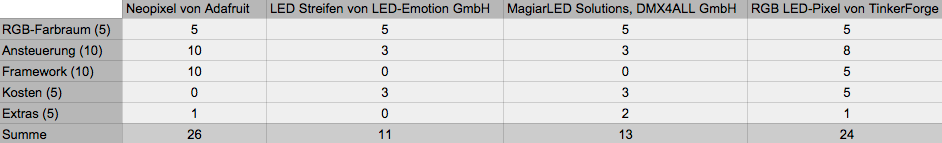
\includegraphics[width=\textwidth]{./data/evaluierung-led.png}
            \captionof{figure}{Ergebnisse der LED-Evaluierung}
        \end{minipage}
\paragraph{Fazit:}
In der Evaluierung schneiden die Produkte von Adafruit und TinkerForge am besten ab. Für eine erste Teststellung werden die einzelnen LED-Pixel von Adafruit aus den USA bestellt (Neopixel). An diesen soll vor allem die Ansteuerung getestet werden. Falls sie sich bewähren, wird für den endgültigen Aufbau auf die LED-Ketten von Tinkerforge zurück gegriffen. 

\subsection{Teststellung}
Für einen ersten Test wurde das in XXX ausgewählte Produkt als einzelne Pixel bestellt. Der Hersteller Adafruit bietet hier 4er-Packungen an. Diese können leicht in eigene Schaltungen eingelötet oder auf Experimentier-Boards gesteckt werden. Bei geringer Anzahl LEDs reicht die 5V-Stromversorgung des Raspberry Pi aus. 
\paragraph{Technische Daten Neopixel:} 
	\begin{itemize}
	\item Maße: 10.2mm x 12.7mm x 2.5mm
	\item Protokollgeschwindigkeit: 800 kHz
	\item Spannung: 5-9VDC  (bei 3,5V gedimmte Helligkeit) 
	\item Strom: 18,5mA / LED, 55mA / Pixel
	\end{itemize}
\paragraph{Framework:}
	\begin{itemize}
	\item RPI\_WS281X (https://github.com/jgarff/rpi\_ws281x)
	\item Sprache: Python
	\item Entwickelt für Raspberry Pi
	\item Vorraussetzung: Python 2.7
	\end{itemize}
\paragraph{Ablauf des Tests:}
\begin{itemize}

\item \textbf{Aufbau der Schaltung}\\
An die einzelnen LED-Pixel wurden Stecker angelötet, damit sie auf das Experimentierboard aufgesteckt werden können. Dann wird die Schaltung nach folgendem Schaltbild verbunden. Wichtig ist, dass beim Raspberry Pi nur Pins verwendet werden können, welche PWM bieten. \\
\begin{minipage}{\linewidth}
            \centering
            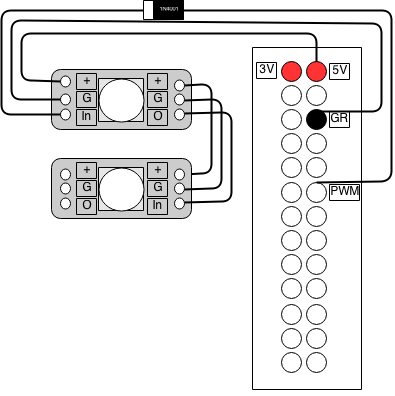
\includegraphics[width=8cm]{./data/TestSchaltungLED.png}
            \captionof{figure}{Schaltung für LED-Test}
        \end{minipage}
\item \textbf{Installation des Frameworks} 
\begin{lstlisting}[caption = Installation Framework ws281x, language=Python, frame=single, breaklines=true,columns=fullflexible, commentstyle=\color{gray}\upshape, captionpos=b, numbers = left]
wget https://github.com/tdicola/rpi_ws281x/raw/master/python/dist/rpi_ws281x-1.0.0-py2.7-linux-armv6l.egg 
sudo easy_install rpi_ws281x-1.0.0-py2.7-linux-armv6l.egg
\end{lstlisting}
\item \textbf{Testcode}

\begin{lstlisting}[caption = Testcode zur Ansteuerung der LEDs, language=python, frame=single, breaklines=true,columns=fullflexible, commentstyle=\color{gray}\upshape, captionpos=b, numbers = left]
from neopixel import * 
	
LED_COUNT   = 4       # Number of LED pixels. 
LED_PIN     = 18      # GPIO pin connected to the pixels (must support PWM!).
LED_FREQ_HZ = 800000  # LED signal frequency in hertz (usually 800khz)
LED_DMA     = 5       # DMA channel to use for generating signal (try 5)
LED_INVERT  = False   # True to invert the signal (when using NPN)

strip = Adafruit_NeoPixel(LED_COUNT, LED_PIN, LED_FREQ_HZ, LED_DMA, LED_INVERT)

strip.begin()
strip.setPixelColor(0, Color(255, 255, 255))
strip.setPixelColor(1, Color(255, 255, 255))
strip.setPixelColor(2, Color(255, 255, 255))
strip.setPixelColor(3, Color(255, 255, 255))
strip.show()
\end{lstlisting}
\end{itemize}
\paragraph{Fazit}
Die einzelnen Pixel sind sehr leicht anzusteuern, unterstützen auch das automatische Abschalten nach einer bestimmten Zeit und haben eine sehr hohe Leuchtkraft. Die Evaluierung hat zu einer guten Produktwahl geführt. \\ 
Nach einer weiteren Nachfrage an Tinkerforge wurde versichert, dass deren LED-Ketten Baugleich zu denen von Adafruit sind. Aufgrund der hohen Versandkosten werden für die endgültige Teststellung die Produkte von Tinkerforge gewählt.

\section{Bewegungssensor} In einem der Modi soll die Beleuchtung durch den Bewegunsmelder ausgelöst werden. Hierfür sind zuverlässige und weitreichende Bewegungssensoren notwendig.
\subsection{Bewertungskriterien}
\begin{itemize}
\item \textbf{Ansteuerung}\\
Die Anbindung an den Raspberry Pi soll möglichst leicht realisierbar sein. Wünschenswert ist, dass der Sensor einfach ein High-Signal bei Bewegungserkennung ausgibt. \\
Gewichtung: 5, KO-Kriterium
\item \textbf{Reichweite}\\
Die Reichweite oder Sensivität des Sensors soll ausreichend und regelbar sein.\\
Gewichtung: 3
\item \textbf{Kosten}\\
Es werden nur die reinen Produktkosten, also ohne Versand und Zoll, bewertet. \\
Gewichtung: 1
\item \textbf{Extras}\\
An dieser Stelle können mögliche Extras eines Herstellers einfließen.\\
Gewichtung: 3
\end{itemize}

\subsection{Evaluierung}
\begin{itemize}
\item \textbf{PIR (MOTION) Sensor, Adafruit}\\
Link: \url{http://www.adafruit.com/product/189}\\
Ansteuerung: Gibt High-Signal an einem Pin aus.\\
Reichweite: 7m, 120 Grad\\
Kosten: 9,95\$ + Versand aus USA\\
Extras: Kabel inklusive\\
\item \textbf{PIR Infrared Motion Sensor (HC-SR501)}\\
Link: \url{https://www.modmypi.com/pir-motion-sensor}\\
Ansteuerung: Gibt High-Signal an einem Pin aus.\\
Reichweite: 5-7m, 100 Grad\\
Kosten: 2,99\$ + Versand aus UK\\
Extras: keine\\
\item \textbf{Infrarot PIR Bewegung Sensor Detektor Modul}\\
Link: \url{http://www.amazon.de/Pyroelectrische-Infrarot-Bewegung-Sensor-Detektor/dp/B008AESDSY/ref=pd\_cp\_ce\_0}\\
Ansteuerung: Gibt High-Signal an einem Pin aus.\\
Reichweite: 7m, 100 Grad\\
Kosten: 5 Stück = 7,66€\\
Extras: keine\\
\end{itemize}
\begin{figure}[h]
\begin{minipage}{\textwidth}
            \centering
            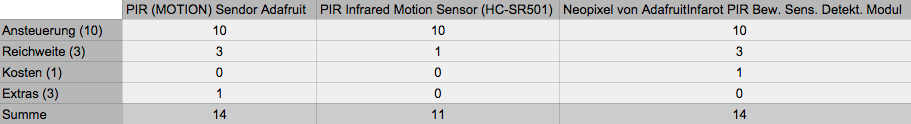
\includegraphics[width=\textwidth]{./data/evaluierung-ms.png}
            \caption{Ergebnisse der Motion-Sensor-Evaluierung}
        \end{minipage}
\end{figure}
\paragraph{Fazit}
Die meisten Infarot-Bewegungssensoren sind von der Bauweise nahezu identisch. Die Unterschiede liegen meist nur in der Empfindlichkeit. Da die Reichweite in diesem Fall nicht von großer Bedeutsamkeit ist, kann eigentlich jedes der Produkte bestellt werden. Auf Ebay und Amazon ist die Anzahl angebotener Sensoren nahezu unbegrenzt, es wurde für die Teststellung also die oben evaluierte Variante von Amazon bestellt. 
\subsection{Teststellung}
Der in Punkt X.X.X gewählte Bewegungssensor wurde beim Hersteller bestellt. In der Teststellung reicht die Stromversorgung des Raspberry Pi. 
\paragraph{Technische Daten Sensor:}
\begin{itemize}
\item Die Empfindlichkeit und Haltezeit kann eingestellt werden
\item Reichweite: ca. 7m
\item Winkel: 100 Grad
\item Spannung: DC 4,5V- 20V
\item Strom: < 50uA
\item Ausgansspannung: High 3V / Low 0V
\item Größe: ca. 32mm x 24mm
\end{itemize}

\paragraph{Ablauf des Tests:}
\begin{itemize}
\item \textbf{Aufbau der Schaltung} \\
Der Sensor wird in der Teststellung direkt vom Raspberry Pi mit Strom versorgt. Für die Datenleitung kann jeder beliebige Pin gewählt werden. 
\item \textbf{Testcode} \\
Um eine Änderung am Datenpin festzustellen werden zwei Variable angelegt: current\_status und previous\_status. Das Programm wird in einer Dauerschleife geschickt, in der bei jedem Durchlauf die beiden Status überprüft. Wenn der neue Status (current\_status) High ist und das vorherige Signal (previous\_state) Low, dann wird eine Bewegung erkannt. Der Code wird mittels Kommentare erklärt.	

\begin{lstlisting}[caption = Testcode zur Bewegungserkennung mit Sensor, language=python, frame=single, breaklines=true,columns=fullflexible, commentstyle=\color{gray}\upshape, captionpos=b, numbers = left]
import RPi.GPIO as GPIO
import time
GPIO.setmode(GPIO.BCM)
# Pin definieren
MOTION_PIN1 = 7
# Diese als Input definieren
GPIO.setup(MOTION_PIN1,GPIO.IN)
# Status definieren um verschiedene Änderungen zu erkennen
Current_State  = 0
Previous_State = 0

try:
	# Loop zur Erkennung einer Bewegung
	# Sensor erkennt Bewegung -> Signal = High
	# Wartet 3 Sekunden und setzt Signal = Low
	while True :
		Current_State = GPIO.input(MOTION_PIN1)
		if Current_State == 1 and Previous_State == 0:
			print "Motion detected!"
			Previous_State=1
		elif Current_State == 0 and Previous_State == 1:
			print "Ready"
			Previous_State=0
		time.sleep(0.01)
	
except KeyboardInterrupt:
	print "Quit"
	GPIO.cleanup()
\end{lstlisting}
Bei der Endversion des Systems sollen mehrere Beweungssensoren integriert werden. Bei Auslösen des ersten Sensors sollen die LEDs angeschaltet werden und nach auslösen eines weiteren Sensors wieder ausgeschaltet werden.  
\end{itemize}

\paragraph{Auswertung}
Das High-Signal des Sensors lässt sich mit dem Raspberry Pi sehr leicht auswerten. Auch die Auswertung von mehreren Sensoren stellt kein Problem da. Das Ergebnis der Evaluierung konnte in dieser Teststellung bestätigt werden. Wichtig für die weitere Implementierung ist, dass die While-Schleife auch abgebrochen werden kann. 



\section{Python-Server und Protokoll} 
\subsection{Protokoll}
Um die LEDs später von einer App aus ansprechen zu können, soll ein auf Strings basierendes Protokoll implementiert werden. Dieses wird in TCP-Paketen übertragen. Hierfür muss als erstes festgelegt werden, welche Informationen übertragen werden sollen: \\
\begin{itemize}
\item Authentifizierung\\
Übertragung eines Passworts. Dieses ist als Hashwert im System gespeichert und kann so überprüft werden. Es wird der SHA-224-Algorithmus eingesetzt.
\item Control\\
Unterscheidung zwischen:\\
	X00: Alle LEDs ausschalten\\
	X01: Eine LED anschalten\\
	X02: LED-Bereich anschalten\\
	X03: Effekt für eine LED\\
	X04: Effekt für LED-Bereich\\
	X05: Effektcode \\\\
Abhängig von diesem Feld werden die nachfolgenden Werte behandelt. 
\item LED-Nummer\\
Falls nur eine LED angesprochen werden soll (Control = X00), so wird hier die Nummer angegeben. Ob sie im gültigen Range liegt wird intern überprüft.
\item Bereich Start\\
Wenn mehrere LEDs gesteuert werden sollen (Control = X01), so wird hier der Beginn des Bereichs angegeben.
\item Bereich Ende\\
Und hier das Ende des Bereichs. 
\item Rot\\
Farbwert Rot 0-255
\item Grün\\
Farbwert Grün 0-255
\item Blau\\
Farbwert Blau 0-255
\item Effekt\\
Es können verschiedene LEDs mit Effekten belegt werden, wie zum Beispiel Aufblitzen oder zeitgesteuertes Ausschalten.
\item Effektcode\\
Hinterlegte, fest programmierte Effekte, zum Beispiel alle LEDs anschalten in weis mit höchster Leuchstärke.
\item Hash\\
Überprüfung ob die Übertragung erfolgreich war, mittels eines Hashwertes. Es wird der SHA-224-Algorithmus eingesetzt.
\end{itemize}
\textbf{Übertragungsbeispiel:}\\
		Protokoll: 	
\begin{lstlisting}[caption = Beispielübertragung des Protokolls, language=python, frame=single, breaklines=true,columns=fullflexible, commentstyle=\color{gray}\upshape, captionpos=b]
auth:control:ledNo:rangeStart:rangeEnd:red:green:blue:effect:effectcode:hash
pass:X01:0:0:49:255:255:255:0:0:xx
Dies würde die LEDs 0 bis 49 einschalten (Farbe weis 255,255,255)
\end{lstlisting}
\subsection{Framework}
Twisted: https://twistedmatrix.com \\
Es wird das Twisted Matrix Framework eingesetzt. Twisted ist eine in Python geschriebene  event-getriebene Netzwerkengine. Die meisten gängigen Protokolle wie TCP, IMAP, SSHv3 und viele mehr werden unterstützt. Somit bietet Twisted die ideale Möglichkeit einen eigenen simplen Server zu implementieren. \\\\
\textbf{Event-Getrieben (event-based):} Die Serveranwendung befindet sich in einer Schleife und wartet auf ein Event. Dieses Event ist in diesem Fall der Connect eines Clients zum Server. Für jeden Connect wird eine neue Instanz angelegt, in welcher empfangene Daten bearbeitet werden können. 

\subsection{Testcode}
\begin{lstlisting}[caption =Testcode Echoserver mit Twisted Framework, language=python, frame=single, breaklines=true,columns=fullflexible, commentstyle=\color{gray}\upshape, captionpos=b, numbers = left]
#!/usr/bin/env python
# Copyright (c) Twisted Matrix Laboratories.
# See LICENSE for details.

from twisted.internet.protocol import Protocol, Factory
from twisted.internet import reactor

### Protocol Implementation

# This is just about the simplest possible protocol
class Echo(Protocol):
	def dataReceived(self, data):
		self.transport.write(data)


	def main():
		f = Factory()
		f.protocol = Echo
		reactor.listenTCP(8000, f)
		reactor.run()

if __name__ == '__main__':
main()
\end{lstlisting}

//TODO ERKLÄRUNG

\subsection{Implementierung}
Im Folgenden wird die Implementierung des Servers näher erläutert. \\\\
	
	// TODO CODE des Servers

\subsection{Klassen und ihre Funktionen}
// TODO
\subsection{Hashfunktion}
Es wird zu zweierlei Zwecken eine Hashfunktion eingesetzt. Zum einen um die Korrektheit der Übertragung zu überprüfen und zum Anderen um ein Passwort zur Authentifizierung verwenden zu können. Dieses wird als Wort übertragen, auf dem Server aber nur als Hash-Wert abgespeichert. Falls es also jemand schafft die Konfirgurationsdatei abzugreifen, so ist der Passworthash nichts wert. 

\section{Verschlüsselung}
\subsection{SSL vs. TLS}
SSL (Secure Sockets Layer) und TLS (Transport Layer Security) sind Protokolle, die Verschlüsselung und Authentifizierung zwischen zwei Kommunikationspartnern bieten. Die beiden Begriffe SSL und TLS werden umgangssprachlich oft als zwei verschiedene Techniken dargestellt, obwohl TLS nur eine Weiterentwicklung von SSL ist. SSL v3 ist die Basis von TLS 1.0. \\
Aufgrund des Alters und einiger Sicherheitslücken wird SSL als unsicher angesehen und soll nicht mehr verwendet werden. Die aktuellste gefundene Lücke ist POODLE, welche das Auslesen von Informationen aus einer verschlüsselten Übertragung erlaubt. Die Weiterentwicklungen TLS 1.1 und 1.2 sind deutlich sicherer und beheben einige sicherheitslücken. \\
Eine Variante von TLS ist das sogenannte STARTTLS, bei dem zuerst ein unsicheres 'hello' an den Server gesendet wird. Falls im Anschluss eine Verbindung erfolgreich Zustande kommt, wird zur sicheren Übertragung gewechselt. \\
Wenn ein Server implementiert wird, so muss er alle Techniken unterstützen, beim Client kann der Entwickler selbst entscheiden. Ein Entwickler sollte immer die höchsten Verschlüsselungstechniken einsetzen. \\

\subsection{Vor- und Nachteile TLS}
Jedes höhrer Protokoll kann über TLS übertragen werden, somit ist die Verschlüsselung unabhängig von der genutzten Anwendung. \\
	Der größte Nachteil besteht darin, dass der Verbindungsaufbau serverseitig sehr rechenintensiv ist. Die Verschlüsselung selbst nimmt, abhängig vom Algorithmus, nur noch wenige Rechenleistung in Anspruch. \\

\subsection{TLS Handshake}
1. Client Hello\\
Übertragung von Verschlüsselungsinformationen vom Client an den Server, wie TLS Version oder Verschlüsselungsmöglichkeiten\\
2. Server Hello \\
Server sendet seine Informationen und legt Verschlüsselung fest. \\
3. Server Key Exchange\\
Server sendet seine Identität in Form seines Zertifikats. \\
4. Client Key Exchange\\
Client legt seinen Pre-Shared-Key fest und überträgt ihn verschlüsselt mit dem public Key des Servers.\\
5. Change Cipher Spec\\
Aus dem PSK wird ein Master-Secret generiert, mit welchem die folgenden Übertragung abgesichert wird. \\
6. Application Data\\
Übertragung der Daten. \\

\subsection{Zertifikat und Key}
Auf dem Raspberry Pi ist OpenSSL in der neuesten Version installiert. Es wird ein selbst-signiertes Zertifikat im 2048 Bit Key erzeugt.\\
1. Private Key erzeugen\\
openssl genrsa -des3 -out server.key 2048\\
2. Certificate Signing Request\\
openssl req -new -key server.key -out server.csr\\
3. Self Signed Certificate\\
Bei einem öffentlichen Server sollte das Zertifikat bei einer CA (Certificate Authority) signiert werden. \\
openssl x509 -req -days 1865 -in server.csr -signkey server.key -out server.crt

\subsection{Beispielcode STARTTLS Server}
An dieser Stelle ist der Beispielcode von Twisted am besten verständlich\\
(Quelle: https://twistedmatrix.com/documents/12.3.0/core/howto/ssl.html)\\
\begin{lstlisting}[caption =Testcode Echoserver mit Twisted Framework, language=python, frame=single, breaklines=true,columns=fullflexible, commentstyle=\color{gray}\upshape, captionpos=b, numbers = left]
from OpenSSL import SSL
from twisted.internet import reactor, ssl
from twisted.internet.protocol import ServerFactory
from twisted.protocols.basic import LineReceiver

class TLSServer(LineReceiver):
    def lineReceived(self, line):
        print "received: " + line

        if line == "STARTTLS":
            print "-- Switching to TLS"
            self.sendLine('READY')
            ctx = ServerTLSContext(
                privateKeyFileName='keys/server.key',
                certificateFileName='keys/server.crt',
                )
            self.transport.startTLS(ctx, self.factory)


class ServerTLSContext(ssl.DefaultOpenSSLContextFactory):
    def __init__(self, *args, **kw):
        kw['sslmethod'] = SSL.TLSv1_METHOD
        ssl.DefaultOpenSSLContextFactory.__init__(self, *args, **kw)

if __name__ == '__main__':
    factory = ServerFactory()
    factory.protocol = TLSServer
    reactor.listenTCP(8000, factory)
    reactor.run()
\end{lstlisting}
Es ist gut zu erkennen, dass die Übertragung nur ausgewertet wird, wenn das Stichwort "STARTTLS" am Anfang der Übertragung enthalten ist. Daraufhin wird mit "READY" geantwortet um dem Client zu signalisieren, dass jetzt der TLS Handshake begonnen werden kann. Im nächsten Schritt läd der Server sein Zertifikat und seinen Key. \\
In der Initmethode der Klasse ServerTLSContext können die Verschlüsselungsdetails festgelegt werden. Im obigen Beispiel wird hier zum Beospiel die TLS Version definiert.  \\

\subsection{Wireshark Trace}

\section{Kamera}
\subsection{PI-Kamera vs. Netzwerkkamera}
Bei Auslösen des System im Überwachungsmodus soll ein aktuelles Bild der Überwachungskamera an das jeweilige Sartphone gepusht werden. Es gibt zwei mögliche Kameratechniken, entweder eine direkt an den Raspberry Pi Angeschlossene oder eine, die im Netzwerk erreichbar ist. 
\paragraph{Raspberry Pi Cam} \\
Die Kameras für den Raspberry Pi können direkt an das Gerät angeschlossen werden. Meistens werden sie direkt über die GPIO Pins verbunden. Der Vorteil dieser Kameras ist, dass sie keine externe Stromversorgung benötigen und durch viele verschiedene Frameworks leicht anpassbar und verwaltbar sind. Der große Nachteil ist allerdings, dass die Kamera an dem Raspberry Pi angeschlossen werden muss, auf welchem auch der Server läuft. Da dieser aber möglich wettergeschützt (im Außenbereich) oder unauffällig (im Innenbereich) angebracht ist, lässt sich von diesen Positionen kaum eine effektive Überwachung realisieren. \\
Als Beispiel wäre ein von der Raspberry Pi Foundation empfohlene Kamera zu nennen: //TODO Beispielkamera
\paragraph{Netzwerkkamera} \\
Eine Netzwerkkamera oder auch IP-Kamera genannt befindet sich im Netzwerk und kann über eine Website oder App eingesehen und gesteuert werden. Der Vorteil ist, dass sie sich irgendwo befinden kann, solange sie im selben Netzwerk ist. Somit kann zum Beispiel eine wetterfeste Kamera im Außenbereich angebracht werden und der Server kann sich im geschützten Innenbereich befinden. \\
Der Nachteil besteht bei IP-Kameras darin, dass es keine einheitliche API zum Abgreifen des Videomaterials gibt. Eine mögliche Lösung wäre das Laden der HTML Seite über einen HTTP-Request und darauffolgend das Ausfiltern des Bildmaterials. Über diese Variante kann aber kein Video sondern nur temporäre Bilder geladen werden. Dies würde aber für eine Notification auf dem Smartphone ausreichen. \\\\
Für dieses Projekt wird eine IP-Kamera aufgrund von oben genannten Vorteilen verwendet.
\subsection{Ansteuerung}
\paragraph{Testcode HTTP-Request}
\paragraph{Implementierung}

\section{Anwendungsstruktur}
\subsection{Klassen und ihre Funktionen}
Die Klasse 'Center' stellt die zentrale Stelle in der Anwendung dar, an der alle Informationen zusammen laufen und verwaltet werden. In der Klasse 'Sensor' werden die einzelnen Bewegungssensoren überwacht. Falls eine Bewegung detektiert wird, so werden in 'Center' die notwendigen Methoden aufgerufen um die LEDs an- oder auszuschalten.\\
Die Klasse 'LED\_Control' verwaltet die eingerichteten LEDs und steuert diese. Hier werden auch die möglichen Effekte gesteuert. Die Methoden in dieser Klasse werden aus der Klasse 'Center' aufgerufen. Ein Zugriff in die andere Richtung ist nicht möglich. \\\\
Alle Serverfunktionaltitäten werden in der Klasse 'Server' bereitgestellt. Hier werden die Daten von Übertragungen empfangen und ausgewertet. Die Prüfung der Korrektheit der einzelnen Protokollbestandteile findet ebenfalls hier statt. Wenn alle Überprüfungen erfolgreich sind, werden die Befehle an 'Center' weiter gegeben und dort ausgeführt. Wenn eine Antwort notwendig ist, zum Beispiel eine Statusabfrage der App an den Server, so werden die Informationen von 'Center' gesammelt und dann von 'Server' verpackt und in korrektem Format an das Mobilgerät gesendet. \\\\
Informationen die für den Betrieb des Systems notwendig sind, werden in der 'Config.ini' gespeichert und können nur über die Klasse 'ConfigReader' abgerufen werden. Es werden Informationen wie Anzahl der LEDs, Passworthash oder Adresse der Netzwerkkamera abgespeichert. Die Konfigurationsdatei wird beim Installationsvorgang erstellt. \\\\
Abrufen von Bildmaterial von der Netzwerkkamera findet ausschließlich über die Klasse 'Cam' statt. Die Klasse ruft die Informationen ab und filtert das Bildmaterial. Somit geben die Methoden der Klasse nur ein Bild zurück. \\\\
In der Klasse 'Status' kann ein Status des Gesamtsystems in der Kommandozeile ausgegeben werden und über 'Log' können Informationen im Logfile gespeichert werden. \\\\
Einzelne Rückgabetypen von Methoden, sowie die Initialisierung von allen Klassen kann mit 'UNIT\_Test' getestet werden. \\\\

\begin{lstlisting}[caption=Ausgabe der Klasse UNIT\_Test, language=python, frame=single, breaklines=true,columns=fullflexible, commentstyle=\color{gray}\upshape, captionpos=b, numbers = left]
root@raspberrypi:/home/timo/Studienarbeit# python UNIT_Test.py 
test_Center (__main__.TestSequenceFunctions) ... ok
test_Effects (__main__.TestSequenceFunctions) ... ok
test_LEDControl (__main__.TestSequenceFunctions) ... ok
test_Sensor (__main__.TestSequenceFunctions) ... ok
test_Server (__main__.TestSequenceFunctions) ... ok
test_Status (__main__.TestSequenceFunctions) ... ok
test_camAdress_MUST_FAIL (__main__.TestSequenceFunctions) ... FAIL
test_camAvaible (__main__.TestSequenceFunctions) ... ok
test_getHashPass (__main__.TestSequenceFunctions) ... ok
test_getMotionPin1 (__main__.TestSequenceFunctions) ... ok
test_getNumberOfLED (__main__.TestSequenceFunctions) ... ok

=============================================
FAIL: test_camAdress_MUST_FAIL (__main__.TestSequenceFunctions)
--------------------------------------------
Traceback (most recent call last):
  File "UNIT_Test.py", line 67, in test_camAdress_MUST_FAIL
    self.assertEqual(resultTest, resultCorrect)
AssertionError: '192.168.2.205' != '123'

--------------------------------------------
Ran 11 tests in 1.873s
\end{lstlisting}
\section{Konfiguration und Installation}
\subsection{Konfiguration}
\subsection{Installation}

\section{iOS App}
\subsection{Konzept}
\subsection{...}
\subsection{...}

\chapter{Praktische Umsetzung}

\chapter{Kostenaufstellung}

\chapter{Fazit}

\addcontentsline{toc}{chapter}{Abbildungsverzeichnis}
\listoffigures

\begin{thebibliography}{xxxxxxxxxxxxxxxxxxx}
 \bibitem[I.]{eventbased}"'SWR Info - Zahlen, Daten, Fakten über den SWR"', \url{http://www.swr.de/unternehmen/unternehmen/kennzahlen/kennzahlen-organisation/-/id=12213420/did=12302978/nid=12213420/eqq46v/index.html}, 13.12.2013
%\bibitem[Thema]{Bezeichner}"'Überschrift"', \url{LINK}, Datum
\end{thebibliography}

 \end{document}

 